% !TEX TS-program = xelatex
\documentclass[10pt]{article}
\usepackage[paperwidth=24cm,paperheight=12cm,margin=0.6cm]{geometry} % 2:1
\pagestyle{empty}

\usepackage{amsmath,amssymb,bm}
\usepackage{kotex}
\usepackage{tikz}
\usetikzlibrary{arrows.meta,positioning,calc}

\begin{document}
	\begin{center}
		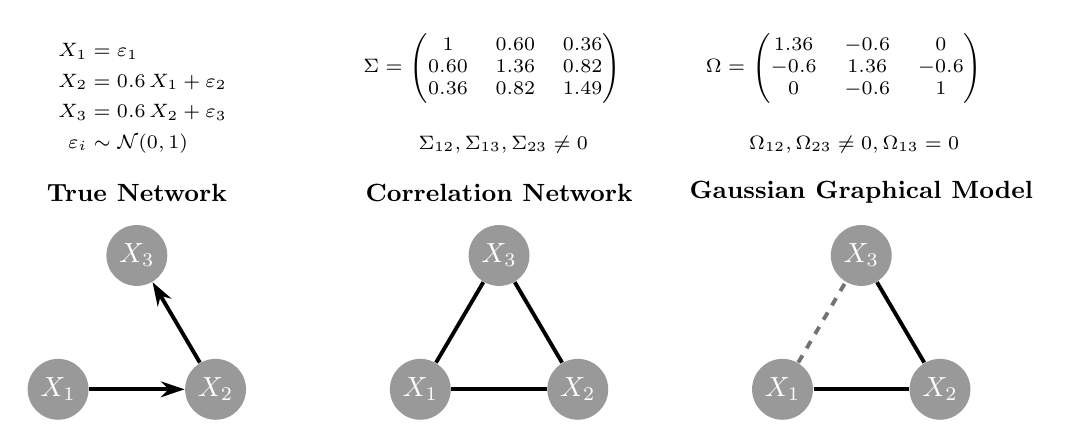
\begin{tikzpicture}[
			node/.style={circle, fill=black!40, text=white, minimum size=22pt, inner sep=0pt, font=\bfseries},
			edge/.style={line width=1.4pt},
			dashededge/.style={edge, dashed, opacity=0.55},
			lab/.style={font=\small, inner sep=1pt, fill=white, fill opacity=0.9, text opacity=1},
			mat/.style={font=\scriptsize, align=left, inner sep=2pt, fill=white, fill opacity=0.95, text opacity=1, rounded corners=2pt}
			]
			
			% --------------------------------------------------------------------
			% SEM block (top)
			% --------------------------------------------------------------------
			\node[align=left, font=\small] (sem) at (-4.2,3.9) {%
				\scriptsize
				$
				\begin{aligned}
					X_1 &= \varepsilon_1\\
					X_2 &= 0.6\,X_1 + \varepsilon_2\\
					X_3 &= 0.6\,X_2 + \varepsilon_3\\
					\varepsilon_i & \stackrel{\text{}}{\sim}\mathcal N(0,1)
				\end{aligned}
				\qquad
				$
			};
			
			\node[mat, anchor=north west] at (-1.8,4.8) {$
				\Sigma=
				\begin{pmatrix}
					1      & 0.60   & 0.36\\
					0.60   & 1.36   & 0.82\\
					0.36   & 0.82  & 1.49
				\end{pmatrix}
				$};
				
				\node[mat, anchor=north west] at (-1.1,3.5) {$
				\Sigma_{12},\Sigma_{13},\Sigma_{23} \neq 0
				$};
			
			\node[mat, anchor=north west] at (2.55,4.8) {$
				\Omega=
				\begin{pmatrix}
					1.36 & -0.6 & 0\\
					-0.6 & 1.36 & -0.6\\
					0 & -0.6 & 1
				\end{pmatrix}
				$};
				
				\node[mat, anchor=north west] at (3.1,3.5) {$
					\Omega_{12},\Omega_{23} \neq 0, \Omega_{13} = 0
					$};
			
			% coordinates (triangle)
			\coordinate (Lx1) at (-5.6,0.2);
			\coordinate (Lx2) at (-3.6,0.2);
			\coordinate (Lx3) at (-4.6,1.9);
			
			\coordinate (x1) at (-1,0.2);
			\coordinate (x2) at (1,0.2);
			\coordinate (x3) at (0,1.9);
			
			\coordinate (Rx1) at ( 3.6,0.2);
			\coordinate (Rx2) at ( 5.6,0.2);
			\coordinate (Rx3) at ( 4.6,1.9);
			
			% LEFT: correlation network
			\node[font=\bfseries] at (-4.6,2.7) {\small True Network};
			
			\node[node] (X1) at (x1) {$X_1$};
			\node[node] (X2) at (x2) {$X_2$};
			\node[node] (X3) at (x3) {$X_3$};
			
			\draw[edge] (X1)--(X2)  {};
			\draw[edge] (X2)--(X3) {};
			\draw[edge] (X1)--(X3)  {};
			
			% LEFT: correlation network
			\node[font=\bfseries] at (-0,2.7) {\small Correlation  Network};
			
			\node[node] (LX1) at (Lx1) {$X_1$};
			\node[node] (LX2) at (Lx2) {$X_2$};
			\node[node] (LX3) at (Lx3) {$X_3$};
			
			\draw[edge, -{Stealth[length=3mm,width=2mm]}] (LX1)--(LX2)  {};
			\draw[edge, -{Stealth[length=3mm,width=2mm]}] (LX2)--(LX3) {};
			
			% RIGHT: GGM
			\node[font=\bfseries] at (4.6,2.7) {\small Gaussian Graphical Model};
			
			\node[node] (RX1) at (Rx1) {$X_1$};
			\node[node] (RX2) at (Rx2) {$X_2$};
			\node[node] (RX3) at (Rx3) {$X_3$};
			
			\draw[edge] (RX1)--(RX2)  {};
			\draw[edge] (RX2)--(RX3)  {};
			\draw[dashededge] (RX1)--(RX3) {};
			
			
		\end{tikzpicture}
	\end{center}
\end{document}